\chapter{给路径加上时间：五次轨迹}
\begin{notebox}
\textbf{目标}\quad 从端点位置、速度、加速度推导五次曲线，理解分段时间与解析采样，再接入理想执行。\\
\textbf{先修}\quad 第 04、11、13 章；多项式求导、链式法则与线性方程。
\end{notebox}

\section{同样走一米，为什么感觉不同}
几何路径只说经过哪里；轨迹还要说何时到达、到达时多快。
先从静止出发，沿 $x$ 轴走 1 m 后静止，分别用 2 s 和 4 s 完成：
\begin{lstlisting}[language=bash]
ros2 run motion2d quintic_demo tmp/ch14_quintic
/usr/bin/python3 scripts/plot_ch14_quintic.py
\end{lstlisting}
图中的位置曲线走过相同距离，较慢的一组将变化摊到更长时间里，因此速度和加速度更小。
下面从端点条件构造这些曲线，并直接对多项式求导，得到任意时刻的速度和加速度。

\begin{figure}[!ht]
\centering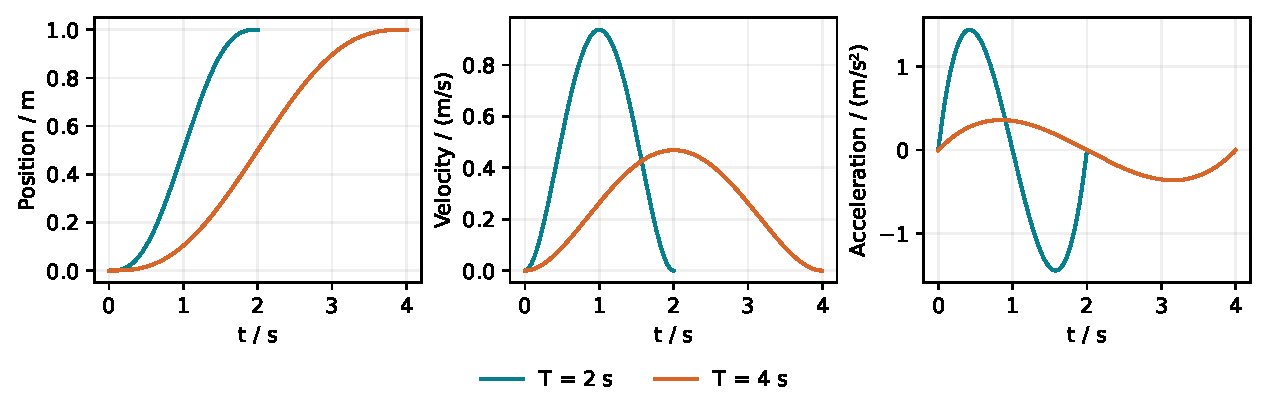
\includegraphics[width=\linewidth]{figures/ch14_scaling.pdf}
\caption{同一几何线段的时间缩放。时长翻倍，速度缩为一半，加速度缩为四分之一。}
\end{figure}

\section{六个边界条件怎样确定六个系数}
\subsection{先用归一化时间写边界}
起点与终点各给位置、速度、加速度，共六个标量条件。
有六个系数的五次多项式正好可以容纳这组条件。二维时对两个坐标分别求解，时长 $T>0$ 共用：
\begin{equation}
p(t)=\sum_{k=0}^{5}c_k t^k,\qquad
\dot p(t)=\sum_{k=1}^{5}kc_k t^{k-1},\qquad
\ddot p(t)=\sum_{k=2}^{5}k(k-1)c_k t^{k-2}.
\end{equation}
$c_k$ 是二维列向量，单位为 $\mathrm{m}/\mathrm{s}^k$。
令 $s=t/T$，将同一条曲线写为 $p(t)=P(s)=\sum_{k=0}^5 b_k s^k$。
$s$ 无量纲，$b_k$ 的单位均为 m；展开 $(t/T)^k$，可知 $c_k=b_k/T^k$。
对时间求导还需用链式法则：
\begin{equation}
\dot p(t)=\frac1T P'(s),\qquad
\ddot p(t)=\frac1{T^2}P''(s).
\end{equation}
因此在 $s=0$ 的三个条件依次给出
\begin{equation}b_0=p_0,\qquad b_1=Tv_0,\qquad b_2=\tfrac12T^2a_0.\end{equation}
在 $s=1$，目标则为 $P(1)=p_1,P'(1)=Tv_1,P''(1)=T^2a_1$。
把已知的前三项移到右边，记剩余量为
\begin{align}
r_0&=p_1-b_0-b_1-b_2,\\
r_1&=Tv_1-b_1-2b_2,\qquad r_2=T^2a_1-2b_2.
\end{align}
三个剩余未知量满足
\begin{equation}
\begin{aligned}
b_3+b_4+b_5&=r_0,\\
3b_3+4b_4+5b_5&=r_1,\\
6b_3+12b_4+20b_5&=r_2.
\end{aligned}
\end{equation}
这些等式对 $x$、$y$ 坐标逐分量成立，可以把向量当作两组相同系数的方程来计算。

\subsection{逐步消元得到代码里的组合}
第二行减去第一行的三倍，第三行减去第一行的六倍，得到
\begin{equation}
b_4+2b_5=r_1-3r_0,\qquad
6b_4+14b_5=r_2-6r_0.
\end{equation}
再用后一式减去前一式的六倍：
$2b_5=r_2-6r_1+12r_0$。回代先求 $b_4$，再求 $b_3$：
\begin{equation}
\begin{aligned}
b_5&=6r_0-3r_1+\tfrac12r_2,\\
b_4&=-15r_0+7r_1-r_2,\\
b_3&=10r_0-4r_1+\tfrac12r_2.
\end{aligned}
\end{equation}
消元时只除以固定非零数，所以任意有限的六个边界值都确定唯一的一组归一化系数。
正时长使最后的 $T^{-k}$ 转换有定义。

\par\noindent\begin{minipage}{\linewidth}
\lstinputlisting[language=C++,linerange={quintic_boundary_begin-quintic_boundary_end},
  includerangemarker=false]{../ros2_ws/src/motion2d/src/trajectory/quintic.cpp}
\end{minipage}\par
代码先填 $b_0,b_1,b_2$，再计算三个残差并回代；最后的 \code{power} 依次取 $1,T,T^2,\ldots,T^5$，
将各列转成秒制系数 $c_k$。
\code{interpolateQuintic} 接收两端的 \code{TranslationState}，返回一个 \code{QuinticPiece}：
正时长加 $2\times6$ 系数矩阵，第一行表示 $x$，第二行表示 $y$，列按\textbf{升幂}排列。

\section{对同一个多项式求各阶导数}
对单项 $c_k t^k$ 求 $r$ 次导数，每次幂次减一，并把原幂次乘到前面：
\begin{equation}
p^{(r)}(t)=\sum_{k=r}^5
\underbrace{k(k-1)\cdots(k-r+1)}_{r\text{ 个因子}}c_k t^{k-r}.
\end{equation}
$r=0$ 时乘积取 1，恢复位置；$r=1,2,3$ 分别为速度、加速度、jerk（加速度的变化率）。
jerk 单位为 $\mathrm{m/s^3}$。高于五阶的导数为零，本章接口接受 0 到 5 阶。

计算多项式可用 Horner 法：从高次项向低次项，反复“乘时间，再加下一系数”。
例如 $d_0+d_1t+d_2t^2+d_3t^3=d_0+t[d_1+t(d_2+td_3)]$。
求导后的系数也可以这样排列，所以同一个循环能计算所有阶数：

\par\noindent\begin{minipage}{\linewidth}
\lstinputlisting[language=C++,linerange={polynomial_derivative_begin-polynomial_derivative_end},
  includerangemarker=false]{../ros2_ws/src/motion2d/src/trajectory/polynomial.cpp}
\end{minipage}\par
内层循环得到上式的 $r$ 个因子，外层从第 5 列往第 $r$ 列走。
最后得到的最低幂是 $t^0$，所以循环在 $k=r$ 时结束。
例如 $x(t)=1+2t+3t^2+4t^3$，则
$\dot x=2+6t+12t^2$、$\ddot x=6+24t$；在 $t=.5$ s，位置为 3.25 m，速度为 8 m/s，加速度为 18 $\mathrm{m/s^2}$。
\textbf{代码练习 ch14-1} 用这个例子核对幂次和乘数。

秒制系数已经包含了 $T^{-k}$，采样器直接代入本段的秒数。
若使用归一化系数 $b_k$ 求导，才需要再按链式法则乘 $T^{-r}$。
两种表示得到同一状态，选择一种约定贯穿保存、发送和采样即可。

\section{静止到静止：形状与峰值都可以手算}
\subsection{从系数得到单调的线段运动}
令 $\Delta p=p_1-p_0$，两端速度与加速度均为零，则 $b_1=b_2=0$、$r_0=\Delta p,r_1=r_2=0$。
代入消元结果便有
\begin{equation}
p(t)=p_0+\Delta p\,h(s),\qquad
h(s)=10s^3-15s^4+6s^5,\quad s=t/T.
\end{equation}
逐次求导并整理：
\begin{align}
h'(s)&=30s^2-60s^3+30s^4=30s^2(1-s)^2,\\
h''(s)&=60s-180s^2+120s^3=60s(1-s)(1-2s),\\
h'''(s)&=60(1-6s+6s^2).
\end{align}
由 $h'(s)\geq0$、$h(0)=0,h(1)=1$，可知 $h$ 在区间内单调从 0 增到 1。
因此位置始终是 $p_0,p_1$ 的非负加权平均，整段保持在线段上。
若该线段属于上一章的安全凸走廊，这种静止到静止的时间分配保持同样的几何包含关系。

\subsection{从导数为零的位置求峰值}
记线段长度 $D=\|\Delta p\|$。速度模长为 $D h'(s)/T$。
极值候选满足 $h''=0$，即 $s=0,1/2,1$；
两端速度为零，中点 $h'(1/2)=30/16=15/8$，所以
\begin{equation}v_{\rm peak}=\frac{15D}{8T}=1.875\frac DT.\end{equation}
加速度模长为 $D|h''|/T^2$。在正、负两半分别寻找极值，令 $h'''=0$：
\begin{equation}
6s^2-6s+1=0\quad\Longrightarrow\quad s=\frac{3\pm\sqrt3}{6}.
\end{equation}
这两点满足 $s(1-s)=1/6$、$|1-2s|=1/\sqrt3$，代入便有
\begin{equation}a_{\rm peak}=\frac{10\sqrt3}{3}\frac D{T^2}.\end{equation}
jerk 的归一化因子 $h'''=360(s-1/2)^2-30$ 在区间内介于 $-30$ 与 60，
故其模长最大值在两端取得：
\begin{equation}j_{\rm peak}=60\frac D{T^3}.\end{equation}
例如 $D=1$ m、$T=2$ s，三个峰值分别为 $.9375$ m/s、$1.4434$ $\mathrm{m/s^2}$、$7.5$ $\mathrm{m/s^3}$。
它们可以直接与第一幅图和后面的实验表核对。

若要为这一特殊线段设置上限 $v_{\max},a_{\max},j_{\max}>0$，将三条峰值不等式分别对 $T$ 求解：
\begin{equation}
T\geq\max\left(\frac{15D}{8v_{\max}},
\sqrt{\frac{10\sqrt3 D}{3a_{\max}}},
\sqrt[3]{\frac{60D}{j_{\max}}}\right).
\end{equation}
这给出了一个可直接实现的时长分配练习。重复点 $D=0$ 时，用正的最短时长生成原地停留段。

\subsection{时间缩放的适用条件}
保持 $P(s)$ 不变，将时长从 $T$ 改为 $\lambda T$，第 $r$ 阶物理导数缩为原来的 $\lambda^{-r}$。
因此时长翻倍时，速度、加速度、jerk 分别乘 $1/2,1/4,1/8$。
这里比较的是\emph{同一归一化形状}。静止边界自动满足这个条件。
若保持非零的物理边界速度 $v_0$ 不变，却重新改变 $T$，则 $b_1=Tv_0$ 也改变，
整条曲线形状可能随之改变；这时应重新求系数后比较。

\section{把若干段接成连续轨迹}
\subsection{连续性是连接处的条件}
把第 $i$ 段终点和第 $i+1$ 段起点设为同一组 $(p,v,a)$，
就使位置、速度与加速度的左极限和右极限相等，称为 $C^2$ 连续。
各段内部是光滑多项式；连接处的 jerk 是否相等，还要比较两边的三阶导数。
例如一维逐点停靠的两段 $0\to1\to3$ m，时长都为 2 s：
连接处两边 $v=a=0$，但左侧 jerk 为 $60\times1/2^3=7.5$，右侧为 $60\times2/2^3=15$ $\mathrm{m/s^3}$。
速度和加速度可以连续，jerk 同时发生跳变。



\code{PolynomialTrajectory} 在相邻段处比较位置、速度、加速度，分别采用对应 SI 单位的 $10^{-7}$ 绝对容差。
最简单的 \code{stopAtWaypoints} 在每个路点设 $v=a=0$，并分配
\begin{equation}
T_i=\max\left(T_{\min},\frac{\|q_{i+1}-q_i\|}{v_{\rm nom}}\right).
\end{equation}
$v_{\rm nom}$ 表示用来计算时长的平均速度参数；在距离项起作用时，峰值为 $1.875v_{\rm nom}$。
每个中间点停下便于观察分段和碰撞几何。第十五、十六章将调整内部速度与加速度，使运动更加连贯。

\begin{figure}[!ht]
\centering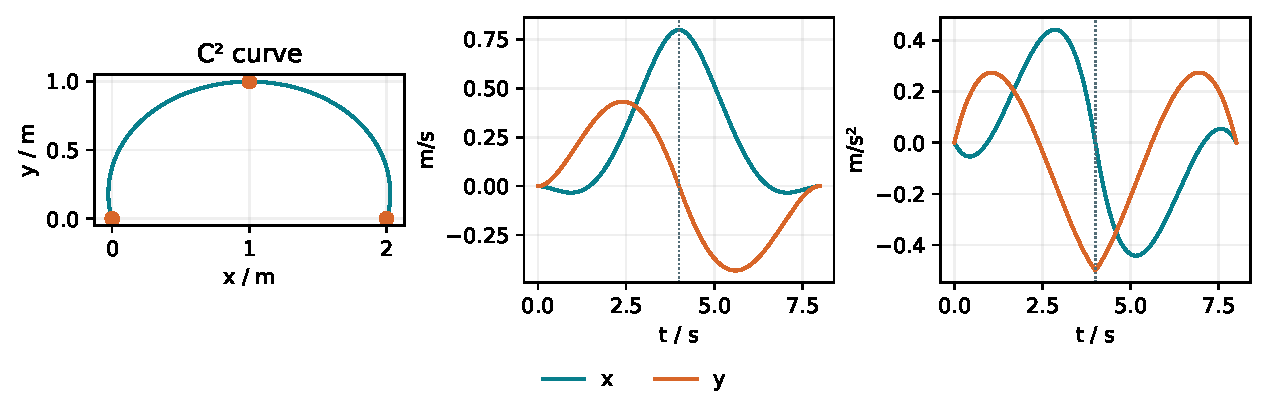
\includegraphics[width=\linewidth]{figures/ch14_join.pdf}
\caption{两个 4 s 分段，连接点 $(1,1)$ m，连接速度 $(0.8,0)$ m/s、加速度 $(0,-0.5)$ $\mathrm{m/s^2}$。
虚线是连接时刻；图形坐标等比例，速度与加速度连续。}
\end{figure}

\subsection{绝对时间、轨迹时间与单段时间}
设绝对开始时刻为 $t_0$，收到查询时刻 $t_{\rm sim}$，先算整条轨迹时间 $\tau=t_{\rm sim}-t_0$。
再减去前面各段时长，得到第 $i$ 段局部时间：
\begin{equation}t_i=\tau-\sum_{k<i}T_k.\end{equation}
多项式 $c_0+c_1t_i+\cdots+c_5t_i^5$ 只接受本段的 $t_i$。
例如 $t_0=.203$ s，两段时长为 $.458,.637$ s，连接与结束时刻为 $.661,1.298$ s。
在仿真时刻 $.700$ s，$\tau=.497$ s，应查询第二段的 $t_2=.039$ s。

\begin{center}
\begin{tikzpicture}[x=6.5cm,y=1cm,>=Stealth]
\draw[->] (0,0)--(1.44,0) node[right]{$t_{\rm sim}$};
\draw[tealblue,very thick] (.203,0)--(.661,0);
\draw[navy,very thick] (.661,0)--(1.298,0);
\foreach \x/\lab in {.203/.203,.661/.661,1.298/1.298} {
 \draw (\x,-.08)--(\x,.08);\node[below] at (\x,-.12){$\lab$ s};
}
\node[font=\small] at (.432,.42){第1段：$T_1=.458$ s};
\node[font=\small] at (.98,.42){第2段：$T_2=.637$ s};
\draw[orange!85!black,->] (.700,.9)--(.700,.08);
\node[above] at (.700,.9){查询 $.700$ s：$t_2=.039$ s};
\end{tikzpicture}
\end{center}
内部连接时刻选择右段，最终时刻选择末段终点。
代码在累计结束时间数组中用 \code{upper_bound} 找第一个严格大于查询时间的边界，正好实现这条规则。
$p,v,a$ 在连接处相同，而 jerk 按所选段给出明确的单侧值。
轨迹前后如何等待与保持，由执行器在下面统一处理。
\subsection{解析参考与显示折线}
/plan/trajectory\_path 是稀疏采样预览：总头记录发布时间，每个 PoseStamped 记录未来执行时间。
真正执行始终使用完整系数；预览折线的密度不影响仿真精度。
RViz 中可同时观察洋红色参考、圆盘与实际轨迹。把预览采样间隔调大，会看到折线变粗糙，
但接收端在同一时刻求出的多项式状态保持一致。


\clearpage
\section{保存系数并复现采样结果}
演示输出 samples.csv、summary.csv 和 coefficients.csv。
系数文件逐行保存案例、段号、时长、坐标轴与六个升幂系数，可用相同采样器重建；不包含 yaw。
平移参考与 yaw 分开指定。全向机器人可以向侧面运动，同时保持机头方向；
阿克曼模型的朝向与速度方向关系已在第四章推导，其轨迹规划在第十六章接入。

\begin{center}\small
\pgfplotstabletypeset[col sep=comma,
columns={case,duration,peak_speed,peak_acceleration,peak_jerk},
columns/case/.style={column name=案例},columns/duration/.style={column name=总时长/s},
columns/peak_speed/.style={column name=速度/(m/s), fixed,precision=4},
columns/peak_acceleration/.style={column name=加速度/(m/s$^2$), fixed,precision=4},
columns/peak_jerk/.style={column name=jerk/(m/s$^3$), fixed,precision=4},
every head row/.style={before row=\toprule,after row=\midrule},
every last row/.style={after row=\bottomrule}]{data/ch14_quintic.csv}
\end{center}
每条完整轨迹在 $t_n=nT_{\rm total}/2000$、$n=0,\ldots,2000$ 处采样，
表中列出这些样本的最大模长。案例 0、1 是上面的 1 m 静止线段，三个解析峰值都可以用来比较采样误差。
例如加速度极值落在 $s=(3\pm\sqrt3)/6$，通常位于两个采样点之间；增加采样密度会更接近它。
案例 2 使用图中的非零连接导数。读取系数文件重新采样，比较连接时刻的左右极限，
再用中心差分检查任意一段内部的解析导数。

\begin{enumerate}
\item \textbf{推导：}从六个静止端点约束推导 $h(s)$，说明 $T$ 翻倍后的各阶导数缩放。
\item \textbf{代码 ch14-1：}完成升幂系数的一阶、二阶导数；避免重复时间缩放。
\item \textbf{实验：}修改中间点速度，比较曲线形状与连续性；解释为何路点安全不足以证明曲线安全。
\end{enumerate}
\section{把轨迹作为完整消息发送}
\begin{lstlisting}[language=bash]
ros2 launch motion2d_bringup ch14.launch.py
ros2 topic pub --once /goal_pose geometry_msgs/msg/PoseStamped \
  '{header: {frame_id: map}, pose: {position: {x: -7.5, y: -8.0}, orientation: {w: 1.0}}}'
ros2 service call /trajectory/execute std_srvs/srv/Trigger '{}'
ros2 topic echo /sim/trajectory_status
\end{lstlisting}
先等待扫描建图与目标规划成功，再调用服务。
点击目标负责产生几何路线；调用服务将当前路线转换为一次完整执行。
trajectory\_node 从区域连接路径取得几何点，从 /odometry 取得选定的定位结果，并用 TF 统一坐标。

motion2d\_interfaces 用分段消息保存系数、用整条轨迹消息保存执行时间和朝向：
\begin{center}\small
\begin{tabular}{ll}\toprule
Trajectory2D 字段 & 明确语义 \\\midrule
header & 发布时间；执行坐标系固定为 odom \\
start\_time & 仿真时钟上的绝对执行起始时刻 \\
pieces & 非空五次分段；每段 duration、x[6]、y[6] \\
yaw & 独立常值朝向，单位 rad \\\bottomrule
\end{tabular}
\end{center}
每段系数以局部秒升幂存储；时长必须有限且为正，连接需满足 $C^2$。
消息转换逐项复制系数与时长，接收端因此能在任意时刻计算参考。
例如 start\_time=0 表示从仿真原点开始；start\_time=.75 s 表示在时钟到达 .75 s 时开始。

\section{把 map 路线固定到 odom}
执行节点在当前里程计时刻查询 $^{odom}T_{map}$，转换所有路点，然后求逐点停靠轨迹。
发布时固定这次变换，整条执行参考随后在 odom 中保持一致。
设转换为 $p_o=Rp_m+d$，若 map 中已有多项式系数，则
\begin{equation}c^o_0=Rc^m_0+d,\qquad c^o_k=Rc^m_k\quad(k\geq1).\end{equation}
因为平移 $d$ 与时间无关，只进入常数项；旋转对每一阶向量都作用相同。
本章代码先变换路点再插值，也得到相应的 odom 曲线。在线重规划与回环衔接将在第十九章处理。
\par\noindent\begin{minipage}{\linewidth}
\lstinputlisting[language=C++,linerange={trajectory_publish_begin-trajectory_publish_end},
  includerangemarker=false]{../ros2_ws/src/motion2d/src/nodes/trajectory_node.cpp}
\end{minipage}\par
\code{transformPoint} 对应点的刚体变换；\code{stopAtWaypoints} 生成各段系数，
\code{lead_} 换成纳秒后加到当前时刻，设置未来的开始时间。
默认平均速度 0.4 m/s、最短分段 0.5 s，执行起点比发布时间晚 0.25 s。
若路线起点与当前位置不一致，拒绝发布并等待新路线；运动中再次发送轨迹由本章执行器明确拒绝。
服务成功表示已发布，最终接收结果看 /sim/trajectory\_status。

\section{用解析参考驱动理想模型}
\subsection{等待、执行与保持}
选择 \code{model=trajectory} 后，仿真器从 /plan/trajectory 接收完整曲线。
这条理想运动分支直接令状态等于参考 $p,v,a$，可先集中观察规划几何和传感器时间。
接收时要求曲线起点与当前位姿一致，两端 $v=a=0$，yaw 连续，开始时刻尚未过去。
这些条件把运动平滑地接到静止等待与终点保持：
\begin{equation}
p_{\rm held}(\tau)=\begin{cases}
p(0),&\tau<0,\\p(\tau),&0\leq\tau\leq T_{\rm total},\\p(T_{\rm total}),&\tau>T_{\rm total}.
\end{cases}
\end{equation}
区间外 $v=a=0$；区间内使用曲线导数。两端的零导数使这条整体参考达到 $C^2$ 连续。
暂停会停止仿真时钟，reset 清空曲线并回到初始状态。
后面的惯性模型将把同样的参考交给控制器，由力与力矩推动机器人接近它。

\subsection{由系数得到步内加速度上界}
仿真每次推进一个时间步，需要检查两端之间的弯曲运动。
第四章已由两次积分推导：若步长为 $h$、步内 $\|\ddot p\|\leq a_{\max}$，
曲线与端点连线之间的偏差不超过
\begin{equation}\delta=\frac{a_{\max}h^2}{8}.\end{equation}
现在曲线是多项式，可以直接从系数求 $a_{\max}$。
对本段局部区间 $0\leq t\leq t_{\max}$，逐项用三角不等式，再利用非负幂的单调性：
\begin{align}
\|\ddot p(t)\|&=\left\|\sum_{k=2}^5 k(k-1)c_k t^{k-2}\right\|\\
&\leq\sum_{k=2}^5 k(k-1)\|c_k\|t^{k-2}
\leq\sum_{k=2}^5 k(k-1)\|c_k\|t_{\max}^{k-2}.
\end{align}
各项单位均为 $\mathrm{m/s^2}$。把向量模长分别相加会忽略项间抵消，所以结果可高于实际峰值，
但整个区间的加速度都被覆盖。一个时间步跨过连接点时，对涉及的每段分别求界，然后取最大值。

\par\noindent\begin{minipage}{\linewidth}
\lstinputlisting[language=C++,linerange={polynomial_sweep_begin-polynomial_sweep_end},
  includerangemarker=false]{../ros2_ws/src/motion2d/src/trajectory/execution.cpp}
\end{minipage}\par
\code{offset} 是当前段在整条轨迹中的起始时间；\code{hi} 将查询终点转换到该段局部时间，
并限制在段末。\code{power} 依次是 $1,t_{\max},t_{\max}^2,t_{\max}^3$，恰好对应加速度中的四项。

例如从 0 到 1 m 的 2 s 静止曲线，非零系数为 $c_3=1.25,c_4=-.9375,c_5=.1875$。
局部时刻不超过 1 s 时，上界为 $7.5+11.25+3.75=22.5$ $\mathrm{m/s^2}$。
取一个长 5 ms、结束不晚于 1 s 的仿真步，得到
$\delta=22.5\times.005^2/8\approx7.03\times10^{-5}$ m。
于是用半径 $r+\delta$ 的圆盘沿端点连线扫掠，就包含原半径 $r$ 沿曲线扫过的全部位置。

\subsection{先确定可推进的时间，再生成传感器样本}
扫掠检查通过后，才接受这次状态推进，并在其中各个传感器采样时刻求解析状态。
检测到碰撞风险时，保持上一个有效状态、冻结时钟，状态为 \code{collision_predicted}。
传感器因此也停在已经接受的时间范围内。
这一步由仿真世界执行，承担物理碰撞裁判的作用；规划仍使用前面建立的观测地图。

\clearpage
\section{在传感器自己的时刻采样}
\begin{lstlisting}[language=bash]
# 默认ch14在运行时
/usr/bin/python3 scripts/check_ch14.py
/usr/bin/python3 scripts/plot_ch14_execution.py
# 停止上一个launch，再运行独立空房间时间实验
ros2 launch motion2d_bringup ch14.launch.py rviz:=false \
  config:=$PWD/ros2_ws/src/motion2d_bringup/config/ch14_time_lab.yaml
/usr/bin/python3 scripts/check_ch14_time.py
\end{lstlisting}

\begin{figure}[!ht]
\centering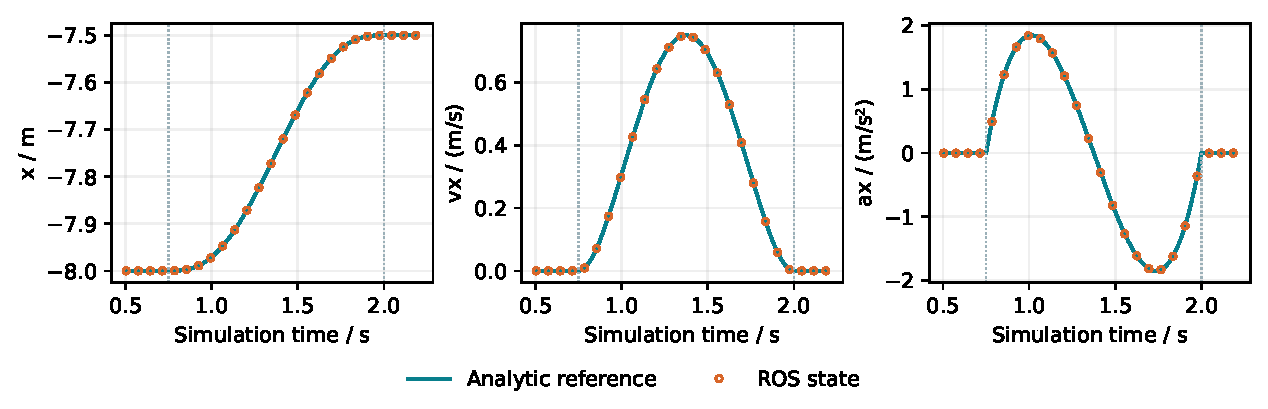
\includegraphics[width=\linewidth]{figures/ch14_execution.pdf}
\caption{实际观测地图上执行半米路线。0.75 s 开始、2 s 结束；实测 p/v/a 与解析参考重合，
用空心点区别采样结果与参考曲线。}
\end{figure}

第一组在真值定位的观测地图上规划 $(-8,-8)\to(-7.5,-8)$ m。
reset 后至 .5 s 发布目标，以默认平均速度 $.4$ m/s 分配时长，得到 $T=.5/.4=1.25$ s。
加上 $.25$ s 提前量，开始与结束时刻便是 $.75$ s 和 $2$ s。
将这些数代入静止线段公式，就能画出图中的参考，并逐条与 ROS 状态消息比较。

第二组用空房间与零噪声，选择 yaw=.4 rad、90 束、137 Hz IMU 和 7 Hz 雷达。
两段轨迹开始、连接、结束时刻为 $.203,.661,1.298$ s，均位于 5 ms tick 之间。
传感器周期也与 tick 不整除：第 29 个 IMU 周期对应
$t=29/137\approx.211678832$ s，它位于 $.210$ 与 $.215$ s 之间。
按前面的时间转换，应在第一段局部 $t_1\approx.008678832$ s 处计算加速度。
随后按第六章的旋转和重力项生成机体系比力，按第五章的射线模型生成雷达距离。

只修改时间戳而沿用 tick 末端状态，会给这个样本代入晚了约 $.003321168$ s 的加速度。
用一个便于手算的局部函数 $x(t_1)=t_1^3$（系数单位 $\mathrm{m/s^3}$）说明：
$\ddot x=6t_1$，上述时差产生约 $.019927$ $\mathrm{m/s^2}$ 的误差。
对一般轨迹，短时误差约为 $j\Delta t$，来自加速度的一阶泰勒展开。
可见采样时刻同时决定消息时间戳和消息数值。

\textbf{练习：}
\begin{enumerate}
\item 用时间实验脚本生成的系数重建 $.700$ s 的第二段状态，确认局部时间为 $.039$ s。
\item 取一条非整步 IMU 消息，分别用采样时刻与 tick 末端时刻求比力，比较差值。
\item 在空房间中发送穿墙曲线，观察最后接受的时刻、碰撞状态，以及之后的消息数量。
解释为何冻结物理时间后，传感器也应停止产生更晚的样本。
\end{enumerate}
进一步的消元、峰值、时间缩放与代码练习见 \path{exercises/ch14}。
